% = = = = = = = = = = = = = = = = = = = = = = = = = = = = = = = = = = = = = = = = = = = = =
% P  R  E  A  M  B  L  E
% = = = = = = = = = = = = = = = = = = = = = = = = = = = = = = = = = = = = = = = = = = = = =
\documentclass[11pt]{article}
\usepackage{amsbsy, amsmath, amssymb, authblk}

%\usepackage{array} 
%\usepackage{algorithm2e}

\usepackage{booktabs, bm}
\usepackage[small,labelfont=bf,up,singlelinecheck=false]{caption}
\usepackage{cancel}
\usepackage{comment}
%\usepackage{fancyhdr}
%\usepackage[default]{lato}
\usepackage[T1]{fontenc}
\usepackage[bottom]{footmisc}
\usepackage{geometry}
\usepackage{graphicx}
\usepackage{hyperref}
%\usepackage[utf8]{inputenc}
%	\inputencoding{latin1}
%	\inputencoding{utf8}
%\usepackage{lettrine}
%\usepackage[sc]{mathpazo}
\usepackage{listings}
\usepackage{lmodern} % Nice fonts?
%\usepackage{mathrsfs}
\usepackage{mathtools} 
%\usepackage{marvosym} % silly bullet-point symbols (misc symbols)
%\usepackage{microtype}
\usepackage{minitoc}         % left in case it is needed elsewhere
\setcounter{secttocdepth}{5} % idem
\usepackage{etoc} % for toc before each section.
%\usepackage{multicol}
\usepackage{needspace}
\usepackage{paralist}
%\usepackage{polynom} 			% typesetting polynomial long division
%\usepackage{setspace}
%	\onehalfspacing 
\usepackage{stmaryrd}  % \llbracket, \rrbracket
\usepackage{tocloft}
\usepackage{xparse} % DeclareDocumentCommand
\usepackage[compact]{titlesec} 		% compact shrinks whitespace around section headings.
\usepackage{ulem} 				% for strikeout \sout command.
%\usepackage{verbatim}

% Muh packagez :)
\usepackage{../Packages/MathCommands}
\usepackage{../Packages/BrandonColors}
\usepackage{../Packages/BrandonBoxes}
\usepackage{../Packages/NoteTaker}

\usepackage{layout} % Type \layout() anywhere to see values of layout frame.
%\usepackage{showframe} % Displays layout frame on all pages
\usepackage{marginnote}
\renewcommand*{\marginfont}{\scriptsize}

\usepackage{tikz}
\usetikzlibrary{arrows, automata, shapes, snakes, positioning}
\usetikzlibrary{bayesnet}

%\setlength{\parskip}{1pt}
%\setlength{\columnseprule}{0.1pt}
%\setlength{\columnsep}{0.6cm}
%\setlength\tabcolsep{0.1cm}
\renewcommand{\arraystretch}{1.2}

\DeclareDocumentEnvironment{definition}{O{-0.5em} o}{
	\IfNoValueTF{#2}{}{\textbf{#2}}
	\vspace*{#1}
	\begin{quote}
		\itshape\small}
	{\end{quote}}

% Title
\title{\vspace{-10mm}\fontsize{24pt}{8pt}\selectfont\textbf{Fall 2016 Course Notes}\vspace*{-4mm}}
% Author
\author{Brandon McKinzie}
% Date
\date{}

\begin{document}
\dosecttoc
\tableofcontents

% ==================================================================================
% ==================================================================================
% ==================================================================================
% BLOGS
% ==================================================================================
% ==================================================================================
% ==================================================================================
\mysection{Blogs}\label{Blogs}


% ======================================================================================
\lecture{Blogs}{Conv Nets: A Modular Perspective}{December 21, 2016}
% ======================================================================================


\p \href{https://colah.github.io/posts/2014-07-Conv-Nets-Modular/}{From this post on Colah's Blog}. 

\myspace The title is inspired by the following figure. Colah mentions how groups of neurons, like $A$, that appear in multiple places are sometimes called \textbf{modules}, and networks that use them are sometimes called modular neural networks. You can feed the output of one convolutional layer into another. With each layer, the network can detect higher-level, more abstract features.
\myfig[0.3\textwidth]{figs/ColahConv2.PNG}
\begin{compactitem}[$\longrightarrow$]
	\item Function of the $A$ neurons: compute certain \textit{features}.
	
	\item Max pooling layers: kind of ``zoom out''. They allow later convolutional layers to work on larger sections of the data. They also make us invariant to some very small transformations of the data.
\end{compactitem}



% ======================================================================================
\lecture{Blogs}{Understanding Convolutions}{December 21, 2016}
% ======================================================================================


\p \href{https://colah.github.io/posts/2014-07-Understanding-Convolutions/}{From Colah's Blog}. 

\p \blue{Ball-Dropping Example}. The posed problem:
\begin{footnotesize}
	\begin{quote}
		Imagine we drop a ball from some height onto the ground, where it only has one dimension of motion. How likely is it that a ball will go a distance c if you drop it and then drop it again from above the point at which it landed?
	\end{quote}
\end{footnotesize}

\begin{figure}[h!]
	\centering
	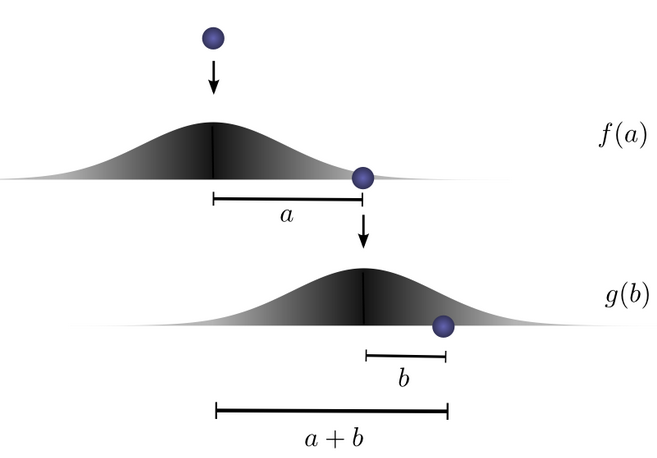
\includegraphics[width=0.35\textwidth]{figs/ColahBall.PNG}
	\hspace{2cm}
	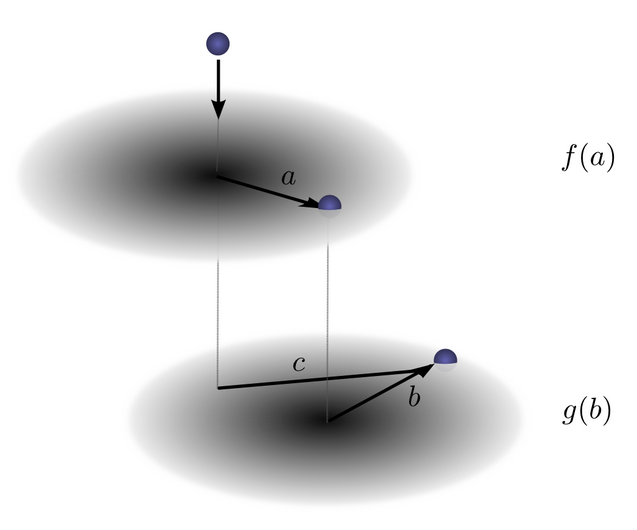
\includegraphics[height=0.25\textwidth]{figs/ColahBall3.PNG}
\end{figure}

From basic probability, we know the result is a sum over possible outcomes, constrained by $a + b = c$. It turns out this is actually the definition of the convolution of $f$ and $g$. 
\begin{align}
\mathrm{Pr(a + b = c)} &= \sum_{a + b = c} f(a) \cdot g(b) \\
(f * g)(c) &= \sum_{a + b = c} f(a) \cdot g(b)\\
&= \sum_a f(a) \cdot g(c - a)
\end{align}

\myspace
\p \blue{Visualizing Convolutions}. Keeping the same example in the back of our heads, consider a few interesting facts. 
\begin{itemize}
	\item \textbf{Flipping directions}. If $f(x)$ yields the probability of landing a distance $x$ away from where it was dropped, what about the probability that it was dropped a distance $x$ from where it \textit{landed}? It is $f(-x)$. 
	
	\myfig[0.3\textwidth]{figs/ColahBall2.PNG}
	
	\item Above is a visualization of one term in the summation of $(f * g)(c)$. It is meant to show how we can move the bottom around to think about evaluating the convolution for different $c$ values. 
\end{itemize}
We can relate these ideas to image recognition. Below are two common kernels used to convolve images with. 
\begin{figure}[h!]
	\centering
	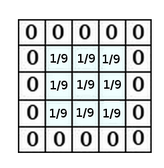
\includegraphics[width=0.15\textwidth]{figs/ColahKernel1.PNG}
	\hspace{2.5cm}
	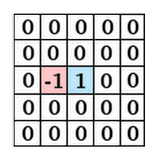
\includegraphics[height=0.15\textwidth]{figs/ColahKernel2.PNG}
\end{figure}

On the left is a kernel for \textit{blurring} images, accomplished by taking simple averages. On the right is a kernel for \textit{edge detection}, accomplished by taking the difference between two pixels, which will be largest at edges, and essentially zero for similar pixels.


\lecture{Blogs}{Deep Reinforcement Learning}{December 23, 2016}

\href{https://www.nervanasys.com/demystifying-deep-reinforcement-learning/}{Link to tutorial} -- Part I of ``Demystifying deep reinforcement learning.'' \\


\p \blue{Reinforcement Learning}. Vulnerable to the \textit{credit assignment problem} - i.e. unsure which of the preceding actions was responsible for getting some reward and to what extent. Also need to address the famous \textit{explore-exploit dilemma} when deciding what strategies to use. 


\myspace
\p \blue{Markov Decision Process}. Most common method for representing a reinforcement problem. MDPs consist of states, actions, and rewards. Total reward is sum of current (includes previous) and \textit{discounted} future rewards:
\begin{equation}
R_t = r_t \gamma(r_{t + 1}
+ \gamma(r_{t + 2} + \ldots)) = r_t + \gamma R_{t + 1}
\end{equation}

\myspace
\p \blue{Q - learning}. Define function $Q(s, a)$ to be best possible score at end of game after performing action $a$ in state $s$; the ``quality'' of an action from a given state. The recursive definition of Q (for one transition) is given below in the \textit{Bellman equation}. 
$$ Q(s, a) = r + \gamma \max_{a'} Q(s', a') $$
and updates are computed with a learning rate $\alpha$ as
$$ Q(s_t, a_t) = (1 - \alpha)\cdot Q(s_{t -1}, a_{t - 1})
+ 	\alpha \cdot (r + \gamma \max_{a'} Q(s'_{t + 1}, a_{t+1}') ) $$

\myspace
\p \blue{Deep Q Network}. Deep learning can take deal with issues related to prohibitively large state spaces. The implementation chosen by DeepMind was to represent the Q-function with a neural network, with the states (pixels) as the input and Q-values as output, where the number of output neurons is the number of possible actions from the input state. We can optimize with simple squared loss:

\myfig{figs/DRL_loss.PNG}

and our algorithm from some state $s$ becomes
\begin{compactitem}
	\item[1.] \textbf{First forward pass} from $s$ to get all predicted Q-values for each possible action. Choose action corresponding to max output, leading to next $s'$.
	
	\item[2.] \textbf{Second forward pass} from $s'$ and again compute $\max_{a'} Q(s', a')$. 
	
	\item[3.] \textbf{Set target output} for each action $a'$ from $s'$. For the action corresponding to max (from step 2) set its target as $r + \gamma \max_{a'} Q(s', a')$, and for all other actions set target to same as originally returned from step 1, making the error 0 for those outputs. (Interpret as update to our guess for the best Q-value, and keep the others the same.)
	
	\item[4.] \textbf{Update weights} using backprop. 
\end{compactitem}


\myspace
\p \blue{Experience Replay}. This the most important trick for helping convergence of Q-values when approximating with non-linear functions. During gameplay all the experience $<s, a, r, s'>$ are stored in a replay memory. When training the network, random minibatches from the replay memory are used instead of the most recent transition. 

\myspace
\p \blue{Exploration}. One could say that initializing the Q-values randomly and then picking the max is essentially a form of exploitation. However, this type of exploration is \textit{greedy}, which can be tamed/fixed with \textbf{$\bm{\varepsilon}$-greedy exploration}. This incorporates a degree of randomness when choosing next action at \textit{all} time-steps, determined by probability $\varepsilon$ that we choose the next action randomly. For example, DeepMind decreases $\varepsilon$ over time from 1 to 0.1. 

\myspace
\p \blue{Deep Q-Learning Algorithm}. 

% https://www.nervanasys.com/wp-content/uploads/2015/12/Screen-Shot-2015-12-21-at-11.23.43-AM-1.png
\myfig[0.75\textwidth]{figs/DRL_alg.PNG}



% ======================================================================================
\lecture{Blogs}{Deep Learning for Chatbots (WildML)}{January 15, 2017}
% ======================================================================================

\p \blue{Overview}. 
\begin{compactitem}
	\item \textbf{Model}. Implementing a retrieval-based model. Input: conversation/context $c$. Output: response $r$. 
	
	\item \textbf{Data}. Ubuntu Dialog Corpus (UDC). 1 million examples of form (context, utterance, label). The label can be 1 (utterance was actual response to the context) or a 0 (utterance chosen randomly). Using NLTK, the data has been . . . 
	\begin{compactitem}[$\rightarrow$]
		\item \green{Tokenized}: dividing strings into lists of substrings.
		\item \green{Stemmed}. \red{IDK}
		\item \green{Lemmatized}. \red{IDK}
	\end{compactitem}
	The test/validation set consists (context, ground-truth utterance, [9 distractors (incorrect utterances)]). The distractors are picked at random\footnote{Better example/approach: Google's Smart Reply uses clustering techniques to come up with a set of possible responses.}
\end{compactitem}

\myspace
\p \blue{Dual-Encoder LSTM}. 

\myfig{figs/DualLSTM.png}

\begin{enumerate}
	\item \textbf{Inputs}. Both the context and the response text are split by words, and each word is embedded into a vector and fed into the same RNN.
	\item \textbf{Prediction}. Multiply the [vector representation ("meaning")] $c$ with param matrix $M$ to predict some response $r'$.
	\item \textbf{Evaluation}. Measure similarity of predicted $r'$ to actual $r$ via simple dot product. Feed this into sigmoid to obtain a probability [of $r'$ being the correct response]. Use (binary) cross-entropy for loss function:
	\begin{align}
	L = -y \cdot \ln(y') - (1 - y) \cdot \ln(1 - y')
	\end{align}
	where $y'$ is the predicted probability that $r'$ is correct response $r$, and $y \in \{0, 1\}$ is the true label for the context-response pair (c, r). 
\end{enumerate}



\myspace
\p \blue{Data Pre-Processing}. Courtesy of WildML, we are given 3 files after preprocessing: train.tfrecords, validation.tfrecords, and test.tfrecords, which use TensorFlow's 'Example' format. Each Example consists of . . . 
\begin{compactitem}
	\item context: Sequence of word ids. 
	\item context\_len: length of the aforementioned sequence.
	\item utterance: seq of word ids representing utterance (response). 
	\item utterance\_len.
	\item label: only in training data. 0 or 1.
	\item distractor\_[N]: Only in test/validation. N ranges from 0 to 8. Seq of word ids reppin the distractor utterance.
	\item distractor\_[N]\_len. 
\end{compactitem}








% ============================================================================================
\lecture{Blogs}{Attentional Interfaces -- Neural Perspective}{April 04, 2017}
% ============================================================================================


{\scriptsize \href{https://theneuralperspective.com/2016/11/20/recurrent-neural-network-rnn-part-4-attentional-interfaces/}{[Link to article]}}


\myspace
\p \blue{Attention Mechanism}. Below is a close-up view/diagram of an attention layer. Technically, it only corresponds to a single time step $i$; we are using the previous decoder state $s_{i - 1}$ to compute the $i$th context vector $c_i$ which will be fed as an input to the decoder for step $i$. 
\myfig[0.5\textwidth]{figs/AttnMech.png}

For convenience, I'll rewrite the familiar equations for computing quantities at some step $i$.
\begin{align}
\mgreen{\text{[decoder state]}} \qquad
s_i &= f(s_{i - 1}, y_{i - 1}, c_i) \\
\mgreen{\text{[context vect]}} \qquad
c_i &= \sum_{j = 1}^{T_x} \alpha_{ij} h_j \\
\mgreen{\text{[annotation weights]}} \qquad
\alpha_{ij} &= \frac{\exp(e_{ij})}{\sum_{k = 1}^{T_x} \exp(e_{ik})} \\
e_{ij} &= a(s_{i - 1}, h_j) 
\end{align}
Now we can see just how simple this really is. Recall that Bahdanau \textit{et al.,} 2015 use the wording: ``$e_{ij}$ \textit{is an alignment model which scores how well the inputs around position $j$ and the output at position $i$ match}.'' But we can see an example implementation of an alignment model above: the $tanh$ function (that's it).








% ================================================================================================
% ================================================================================================
% ------------------------------------- A P P E N D I X ------------------------------------------
% ================================================================================================
% ================================================================================================

%\clearpage

% ==================================================================================
% ==================================================================================
% ==================================================================================
% BLOGS
% ==================================================================================
% ==================================================================================
% ==================================================================================
\mysection{Appendix}\label{Appendix}


\appendixsection{Common Distributions and Models}

\p \blue{Continuous Distributions}.\marginnote{
	$$ (\forall n \in \mathbb{Z}^+)  \Gamma(n) = (n - 1)!   $$
	$$ \Gamma(z) = \int_0^\infty x^{z-1} e^{-x} \mathrm{d}x $$	}

\begin{tabular}{l | l | l}
	Distribution & Density Function & Notation \\ \hline \hline 
	Gaussian
	& $p(\theta) = (2\pi)^{-d/2} \det \lr{ \matr{\Sigma}  }^{-1/2} e^{  -\onehalf (\vec x - \vec \mu)^T \minv{\Sigma} (\vec x- \vec \mu)   }$ 
	& $\theta \sim \Gauss{\vec \mu , \matr \Sigma}$ \\ \hline
\end{tabular}

Distributions with support $\theta > 0$:

\begin{tabular}{l | l | l}
	Distribution & Density Function & Notation \\ \hline \hline 
	Chi-Square 
		& $p(\theta) = \frac{2^{-\nu/2}}{\Gamma(\nu/2)} \theta^{\nu/2 - 1} e^{-\theta/2}$ 
		& $\theta \sim \chi_{\nu}^2$ \\ \hline 
	Gamma 
		&	$p(\theta) = \frac{\beta^{\alpha}}{\Gamma(\alpha)} \theta^{\alpha - 1} e^{-\beta\theta}$
		& $\theta \sim \text{Gamma}(\alpha, \beta)$ \\ \hline
	Inverse-gamma 
		& $p(\theta) = \frac{\beta^{\alpha}}{\Gamma(\alpha)} \theta^{- \alpha - 1} e^{-\beta / \theta}$
		& $\theta \sim \text{Inv-gamma}(\alpha, \beta)$ \\ \hline 
	Inverse-chi-square 
		& $p(\theta) = \frac{2^{-\nu/2}}{\Gamma(\nu/2)} \theta^{- \nu/2 - 1} e^{-\inv{2\theta}}$ 
		& $\theta \sim \text{Inv-} \chi_{\nu}^2$ \\ \hline 
\end{tabular}

Distributions with support $\theta \in [0, 1]$:

\begin{tabular}{l | l | l}
	Distribution & Density Function & Notation \\ \hline \hline 
	Beta 
		& $p(\theta) =  \frac{\Gamma(\alpha + \beta)}{\Gamma(\alpha) + \Gamma(\beta)}  \theta^{\alpha - 1}(1 - \theta)^{\beta - 1} $ 
		& $\theta \sim \text{Beta}(\alpha, \beta)$ \\ \hline
	Dirichlet 
		& $p(\theta) =  \frac{\Gamma(\sum_k \alpha_k)}{\prod_k \Gamma(\alpha_k)} \prod_k \theta_k^{\alpha_k - 1}, ~~ \sum_k \theta_k = 1$ 
		& $\theta \sim \text{Dirichlet}(\alpha_1, \ldots, \alpha_K)$ \\ \hline 
\end{tabular}

\myspace
\p \blue{Discrete Distributions}.

\begin{tabular}{l | l | l}
	Distribution & Density Function & Notation \\ \hline \hline 
	Bernoulli 
		& $p(x; \theta) = \theta^{\ind_{x=1}} (1 - \theta)^{\ind_{x=0}}$ 
		& $X \sim Ber(\theta)$ \\ \hline  
	Binomial 
		& $p(x; n) = \binom{n}{x} p^x (1 - p)^{n - x}$ 
		& $x \sim \text{Bin}(n, p)$ \\ \hline  
	Multinomial 
		& $p(x_1,\ldots,x_k; n) = \frac{n!}{\prod_i^k x_i!} \prod_i^k p_i^{x_i}  $ 
		& \\ \hline
\end{tabular}


\myspace
\p \blue{Logistic Regression}. Perhaps the simplest \textit{linear method}\footnote{We say a classification method is \textit{linear} if its \textbf{decision boundary is linear}.} for classification is \green{logistic regression}. Let $K$ be the number of classes that $y$ can take on. The model is defined as
\graybox{
	\Prob{y = k \mid \vec x} &= \frac{\exp(\vec[k]{\theta}^T \vec x)}{1 + \sum_{\ell = 1}^{K - 1} \exp(\vec[\ell]{\theta}^T \vec x) }, \quad \text{for } 1 \le k \le K - 1 \\
	\Prob{y = K \mid \vec x} &= \frac{1}{1 + \sum_{\ell = 1}^{K - 1} \exp(\vec[\ell]{\theta}^T \vec x) }
}
and we often denote $\Prob{y = k \mid \vec x}$ under the entire set of parameters $\matr{\theta}$ simply as $p_k(\vec x; \matr{\theta})$ or just $p_k(\vec x)$. The decision boundaries are the set of points in the domain of $\vec x$ for which some $p_k(\vec x) = p_{j \ne k}(\vec x)$. Equivalently, the model can be specified by $K-1$ log-odds or logit transformations of the form
\begin{align}
	\log\left(  \frac{p_i(\vec x)}{p_K(\vec x)} \right) &= \vec[i]{\theta}^T \vec x
	\quad \text{for } 1 \le i \le K - 1
\end{align}
Also note that the parameter vectors are orthogonal to the K-1 decision boundaries. For any $x, x'$ on the decision boundary defined as the set of points $\{x: p_a(x) = p_b(x) \}$, we know that the vector $x - x'$ is parallel to the decision boundary (by definition), and can derive
\begin{align}
	\frac{p_a(x)}{p_b(x)} &= 1 = \exp(\theta_a^T x - \theta_b^T x) \implies \theta_a^T x = \theta_b^T x \\
	\therefore \theta_a^T (x-x') &= \theta_b^T (x - x') = 0
\end{align}
and thus $\theta_a$ and $\theta_b$ are both perpendicular to the decision boundary where $p_a(x) = p_b(x)$. 


\appendixsection{Math}

\subsub{Jargon}

Fancy math definitions/concepts for fancy authors who require fancy terminology.
\begin{compactitem}
	\item \green{Support}. Sloppy definition you'll see in most places: The \textit{set-theoretic support} of a real-valued function $f : X \mapsto \R$ is defined as 
	$$
		\text{supp}(f) \triangleq \{x \in X: f(x) \ne 0\}
	$$
	Note that Wikipedia is surprisingly sloppy with how it defines and/or uses support in various articles. After some digging, I finally found the \href{https://www.wikiwand.com/en/Support_(mathematics)#/In_probability_and_measure_theory}{formal definition} for probability and measure theory:
	\begin{definition}
		If $X : \Omega \mapsto \R$ is a random variable on $(\Omega, \mathcal F, P)$, then the \textbf{support} of $X$ is the smallest closed set $R_X \subset \R$ such that $P(X \in R_X) = 1$. 
	\end{definition}
	
	\item \green{Infimum and Supremum}. The fancy-math way of saying minimum and maximum. Yes, I recognize that these are important in certain (usually rather abstract) settings, but often in ML it is used when sup means exactly the same thing as max, but the authors want to look sophisticated. Here I'll give the \href{https://www.wikiwand.com/en/Infimum_and_supremum#/Formal_definition}{formal definition} for $\sup$. You have a partially ordered set\footnote{A partially ordered set $(P, \le)$ is a set of elements such that element $i$ is less than or equal to element $i + i$.} $P$, and are for the moment checking out some subset $S \subseteq P$. Someone asks you, ``hey, give me an \textit{upper bound} of $S$.'' You just gotta find \textit{some} $b \in P$ (the larger/global set) that is greater than or equal to every element in $S$. The person then comes back and says ``ok no, I need the \textit{supremum} of $S$.'' Now you need to find the \textit{smallest} value out of all the possible upper bounds. 
	\myfig[0.5\textwidth]{figs/supremum.png}
	
	Hopefully it is clear why this is only relevant in real-valued cases where the ``edges'' aren't well-defined. 
	
	\item \green{Probability Measure}. Informal definition: a probability distribution\footnote{See \href{https://math.stackexchange.com/a/1073804}{this great answer} detailing how the difference between ``measure'' and ``distribution'' is basically just context.}. Formal definition: a function $\mu: \alpha \mapsto \R[0, 1]$ from events to scalar values, where $\mu(\alpha) = 1$ if $\alpha = \Omega$ (the full space) and $\mu(\varnothing) = 0$. Also $\mu$ must satisfy the countable additivity property: $\mu(\cup_{i} \alpha_i) = \sum_{i} \mu(\alpha_i)$ for pairwise disjoint sets $\{\alpha\}_i$. 
\end{compactitem}




\subsub{Linear Algebra} 

Feeling like I need a quick recap from my adv. linalg course and an area where I can ramble my interpretations. In what follows, let $V$ and $W$ be vector spaces over some field $F$.

\begin{definition}[-1em][Linear Transformation]
	A function $T: V \mapsto W$ is called a \green{linear transformation} from $V$ to $W$ if $\forall x,y \in V$ and $\forall c \in F$:
	\begin{compactitem}
		\item $T(x + y) = T(x) + T(y)$. 
		\item $T(cx) = cT(x)$. 
	\end{compactitem}
\end{definition}
Now suppose that $V$ and $W$ have ordered bases $\mathcal V = \{v_1, \ldots, v_n\}$ and $\mathcal W = \{w_1, \ldots, w_m\}$, respectively. Then for each basis vector $v_j$, there exist unique scalars $a_{ij} \in F$ such that
\begin{align}
	T(\vec[j]{v}) &= \sum_{i=1}^m a_{ij} \vec[i]{w} 
\end{align} 
Remember that each $v_j$ and $w_i$ are members of a \textit{vector} space (they are not scalars). And also be careful to not associate the representation of any vector space element with its coordinate vector relative to a specific ordered basis, which \textit{itself is a different linear transformation from some $V \mapsto F^n$}. Keep it abstract.

\begin{definition}[-1em][Matrix Representation of a Linear Transformation]
	We call the $m \times n$ matrix $A$ defined by $A_{ij} = a_{ij}$ the \green{matrix representation of $T$} in the ordered bases $\mathcal V$ and $\mathcal W$ and write $A = [T]_{\mathcal V}^{\mathcal W}$. If $V = W$ and $\mathcal V = \mathcal W$, then $A =  [T]_{\mathcal V}$. 
\end{definition}
Given this definition, I think it's wise to interpret matrix representations by the column-vector point of view. Each column vector $[T(v_j)]_{\mathcal W}$, read as ``the coordinate vector of $T(v_j)$ relative to ordered basis $\mathcal W$,'' tells you how each basis vector $v_j$ in domain $V$ gets mapped to a [coordinate] vector in output space $W$ [relative to a given ordered basis $\mathcal W$]. For some reason, my brain has always had a hard time with the fact that the matrix row indices $i$ correspond to output space, while the column indices $j$ represent the input space. The easiest way (I think) to help ground this the right way is to remember that $L_A(x) \triangleq A x$, i.e. the operator view. At the same time, notice how the effect of $Ax$ is to take successive linear combinations over each element of $x$. 

\begin{align}
	\matr A \vec x = \jnsum T(\vec[j]{v}) x_j
\end{align}

I just realized another reason why the interpretation felt backwards to my brain: when we are taught matrix multiplication, we do the computations $Ax$ in our heads ``row by row'' along $A$, taking inner products of the row with $x$, so I've been taught to think of the rows as the main ``units'' of the matrix. I'm not sure how to fix this, but notice that the matrix is basically just a blueprint/roadmap/whatever you want to call it for taking coordinate vectors in one basis to coordinate vectors in another basis. It's really important to remember the coefficients of $A$ are intimately tied to the input/output bases.  \\

\red{AHA}. I've been thinking about this all wrong. For the longest time, I've been trying to force an interpretation of matrix multiplication that ``feels'' like scalar multiplication. I realize now that this is going about it all the wrong way. \textit{Matrix multiplication need only be considered from the lens of a linear transformation}. After all, that's exactly the purpose of matrices anyway! It's so glaringly obvious from the paragraphs above, but I guess I never took them seriously enough. Matrices are simply convenient ways for us to write down linear transformations on vectors in a given [ordered] basis. The jth column of the matrix defines how the original jth basis vector is transformed. \red{AHA} (again). Now I see why I missed this crucial connection -- \textit{everything above focuses on the formal definition of input ordered basis $\beta$ to output ordered basis $\gamma$, but 99 percent of the time in real life we have either $\beta \subset \gamma$ or $\gamma \subset \beta$ (we usually are mapping from $\R^n$ to $\R^m$). } For example, let $\matr A \in M^{m \times n}$ and $\vec x \in \R^{n}$; the following is \underline{always} true:
\begin{align}
	\matr A \vec x
		&= L_A(\vec x) \\
		&= \begin{bmatrix}
			L_A(\vec[1]{\hat e}) & L_A(\vec[2]{\hat e}) & \cdots & L_A(\vec[n]{\hat e})
		\end{bmatrix}
		\vec x \\
		&= \sum_{i = 1}^{n} L_A(\vec[i]{\hat e}) x_i
\end{align}
This viewpoint is painfully obvious to me now, but I guess I hadn't thought deeply enough about the implications of the definition of a linear transformation, and I \textit{definitely} took the \textbf{representation} of a matrix way too seriously, rather than focusing on its \textbf{sole purpose}: provide a convenient way to write down linear transformations. For example, the above is actually a direct consequence of the definition of a L.T. itself:
\begin{align}
	L_A(\vec x)
		&= L_A(x_1 \vec[1]{\hat e} + \cdots + x_n \vec[n]{\hat e}) \\
		&= x_1 L_A(\vec[1]{\hat e}) + \cdots + x_n L_A(\vec[n]{\hat e})
\end{align}
Time to really nail in the understanding. I also remember getting screwed up trying to think about \textit{ok, so how do I conceptualize of the ith element of $\vec x$ \textit{after} the transformation? It's just a bunch of summed up goobley-gook!}. On one hand, yes that's true, but focus on the following before/after representations of $\vec x$ to make your life easier:
\begin{align}
	\vec{x} {\triangleq} \sum_i^n x_i \vec[i]{\hat e}
	\quad \xrightarrow{~~ Ax ~~} \quad
	L_A(\vec x) {\triangleq} \sum_i^n x_i L_A(\vec[i]{\hat e})
\end{align}

\myspace
\blue{Matrix-Matrix Multiplication}. Continuing with the viewpoint that a matrix is nothing more than a convenient way to represent a linear transformation, recognize that any matrix multiplication $A B$ represents a linear transformation itself, defined as $T := T_A \circ T_B$, the composition of $A$ and $B$. 

\myspace
\p \blue{Matrix Multiplication and Neural Networks}. Let's use the previous interpretations in the context of neural networks. A basic feedforward network with one hidden layer will compute outputs $\vec o$ given inputs $\vec x$, each of which are vectors of possibly different dimension:
\begin{align}
\vec{o}(\vec x) 
	&= \matr{W}^{(o)} \vec{\phi}(\vec x) \\
\vec{\phi}(\vec x)
	&= \matr{W}^{(h)} \vec x
\end{align}
where $\matr{W}^{(o)}$ and $\matr{W}^{(h)}$ are the output and hidden parameter matrices, respectively. We already know that we can interpret each columns of these matrices as how the input basis vectors get mapped to the hidden or output space. However, since we usually think of the parameter matrices as representing the weighted edges of a network, we often think in terms of individual units. For example, the $i$th unit of the hidden layer vector $\vec h$ is given by $h_i = \sum_j^{n_{in}} W_{ij} x_j = \langle \matr[i,:]{W} ,  \vec x \rangle$. One interesting interpretation is that the $i$th element of $\vec h$ is a \textbf{projection}\footnote{This is informally worded. See the footnotes in the dot products section to understand why the element is technically just the result of a transformation (a projection would require re-mapping the scalar back to the space that $\matr[i, :]{W}$ lives (input space)).} of the input $\vec x$ onto the $i$th row of $\matr W$. This is of course true for any linear transformation; we can always think of the elements of the transformed vector as the result of projections of the original vector along a particular direction.

\myspace
\p \blue{Determinants}. $\det A$ is the volume of space that a unit [hyper] cube is mapped to. Starting with the simplest non-trivial case, let $A \in M^{2 \times 2}$, and define $A$ s.t. it simply scales the basis vectors (zero rotation). In other words, $A_{i, j{\ne}i} := 0$. In this case, $\det{A} = a_{11}a_{22}$, which is the area enclosed by the new scaled basis vectors. Skipping straight to the general case of [necessarily square] matrix $A \in M^{n \times n}$ using Einstein summation notation and the Levi-Cevita symbol\footnote{Recall that 
	\begin{align}
		\varepsilon_{i_1, \ldots, i_n}
			&\triangleq \begin{cases}
				+1 & \text{if }(i_1, \ldots, i_n)\text{ is even perm of }(1, \ldots, n) \\
				-1 & \text{if }(i_1, \ldots, i_n)\text{ is odd perm of }(1, \ldots, n) \\
				0 & \text{otherwise}
			\end{cases}
	\end{align}
	Note that this implies equal-to-zero if any of the indices are equal.
}:
\begin{align}
	\det A
		&\triangleq \varepsilon_{i_1, \ldots i_n} a_{1, i_1} \ldots a_{n, i_n}
		= \varepsilon_{i_1, \ldots i_n} \prod_{j=1}^{n} a_{j, i_j}
\end{align}
Consider that if $\det A = 0$, then $T_A$ ``squishes'' the volume of space in such a way that we essentially lose one or more dimensions. Notice how it only takes \textit{one} lost dimension, since the volume of any region in $\R^n$ is zero unless there is \textit{some} amount in all dimensions (e.g. a cube with zero width has zero volume, regardless of its height/depth). It's also interesting to consider the relationships here with the invertible matrix theorem (defined a few paragraphs below). Having the intuition that determinants can be thought of as a change-in-volume makes it much more obvious why the equivalence statements of the invertible matrix theorem are indeed equivalent. 

\myspace
\p \blue{Dot Products and Projections}. First, recall that a projection is \textit{defined} to be a \textbf{linear} transformation $P$ that is idempotent ($P^n = P$ for $n \ge 1$). Also, note that what you generally think of as a projection is technically an \textit{orthogonal projection}\footnote{The more general definition uses wording ``projection of vector $\vec x$ \textit{along $\vec k$} onto $\vec m$'', where the distinction is shown in italics. An orthogonal projection implicitly defines $\vec k$ as its null space; for any $\alpha \in \R$, an orthogonal projection satisfies $P( \alpha \vec k) = \vec 0$}. \\

\Needspace{15\baselineskip}
Here we'll show the intimate link between the dot product and [orthogonal] projection. Let $P_{\vec u}$ define the [orthogonal] projection onto some \textbf{unit} \textit{vector} $\vec u \in \R^n$ (more generally, we could project onto a subspace instead of a single vector\footnote{And technically, you don't project onto a \textit{vector}, but rather you project onto a \textit{line}, which is itself technically a subspace of 1 dimension. Yada yada yada.}). We can re-cast this as a linear transformation $T_{\vec u} : \R^n \mapsto \R$ (technically not a \textit{projection}, which would require re-mapping the output scalar back to $\R^n$). We interpret the scalar output of $T_{\vec u}(\vec x)$ as the coordinate along the line spanned by $\{ \vec u \}$ that input vector $\vec x$ gets mapped to. But wait, didn't we just talk a bunch about how to represent/conceptualize of the matrix representation of a transformation? Yes, we did. Well then, what would the matrix representation of $T_{\vec u}$ look like? Don't forget that we've defined $|| \vec u || = 1$.
\begin{align}
	\left[  T_{\vec u}  \right]_{\R^n}^{\R}
		&= \begin{bmatrix}
			u_1 & \cdots & u_n 
		\end{bmatrix} \\
	T_{\vec u}(\vec x) 
		&= \sum_i^n u_i x_i \\
	\longrightarrow ~~	&= \vec x \dotp \vec u
\end{align}
Furthermore, since linear transformations satisfy $T(c \vec x) = c  T(\vec x)$ by definition, the final result is true even when $\vec u$ is not a unit vector. 



\myspace
\blue{Invertibility and Isomorphisms}. A function is invertible IFF it is both one-to-one and onto (i.e. bijective). Recall that $rank(T)$ is the dimensionality of the range of $T$, which is the subspace of $W$ that $T$ maps to. 
\begin{definition}
	Let $T: V \mapsto W$ be a linear transformation, where $V$ and $W$ are finite-dimensional spaces of \underline{equal dimension}. Then $T$ is invertible IFF rank$(T)$ = dim$(V)$. 
\end{definition}
For any invertible functions $T$ and $U$:
\begin{compactitem}
	\item $(TU)^{-1} = U^{-1} T^{-1}$. One easy way to show this is
	\begin{align}
		(TU)U^{-1}T^{-1}(x)
			&= T(UU^{-1})T^{-1}(x)
			= TT^{-1}(x)
			= x
	\end{align}
	
	\item $(T^{-1})^{-1} = T$. The inverse of $T$ is itself invertible. 
\end{compactitem}
\vspace{1em}

% --- SCHURS COMPLEMENT -----
\newcommand{\scomp}[2]{\matr{#1} / \matr{#2}}
\newcommand{\scompinv}[2]{\left( \scomp{#1}{#2} \right)^{-1}}
\Needspace{10\baselineskip}
\begin{definition}[-1em][Inverse of a partitioned matrix]
	Consider a general partitioned matrix,
	\begin{align}
		\matr M &= \begin{pmatrix}
			\matr E & \matr F \\
			\matr G & \matr H 
		\end{pmatrix}
	\end{align}
	where $\matr E$ and $\matr H$ are invertible. Then
	\begin{align}
		\minv{M} &= \begin{pmatrix}
			\scompinv{M}{H} & - \scompinv{M}{H} \matr F \minv{H} \\
			\minv{E} + \minv E \matr F \scompinv{M}{E} \matr G \minv{E} &
			\scompinv{M}{E}
		\end{pmatrix}\\
		\text{where}\quad
		\scomp{M}{H}
			&\triangleq \matr E - \matr F \minv H \matr G \\
		\scomp{M}{E}
			&\triangleq \matr H - \matr G \minv E \matr F
	\end{align}
	where $\scomp{M}{H}$ denotes the \green{Schur complement} of $\matr M$ w.r.t. $\matr H$. 
\end{definition}

\Needspace{15\baselineskip}
\begin{definition}[-1em][Invertible Matrix Theorem]
	Let $\matr A$ be a square $n \times n$ matrix over some field $K$. The following statements are equivalent (I'll group statements that are nearly identical, too):
	\begin{itemize}
		\item The ones I consider useful:
		\begin{compactenum}
			\item $\matr A$ is invertible.
		
			\item $\matr A$ is row-equivalent (and thus column-equivalent) to $\matr[n]{I}$. 
			
			\item $\det \matr A \ne 0$. 
			
			\item $\text{rank}(\matr A) = n$. 
			
			\item The columns of $\matr A$ are linearly independent. They span $K^n$. $\text{Col}(\matr A) = K^n$. 
			
			\item The transformation $T(\vec x) = \matr A \vec x$ is a bijection from $K^n$ to $K^n$. 
		\end{compactenum}
		
		\item The rest:
		\begin{compactenum}	
			\item $\matr A$ has $n$ pivot positions.
			
			\item $\matr A$ can be expressed as a finite product of elementary matrices.
		\end{compactenum}


	\end{itemize} 
\end{definition}

\textbf{Relationships between $\matr X$ and $\matr X^\top \matr X$}. If $\matr X \in \R^{n \times d}$ has full column rank, i.e. the $d$ columns are linearly independent vectors in $\R^n$ (note that this implies $d \leq n$), the $\matr X^\top \matr X$ is positive definite and thus invertible. 

\vspace{1em}
\rule[0.5ex]{\linewidth}{1pt}

\myspace
\p \blue{Understanding correlation vs independence}. 
\begin{compactitem}
	\item Two \textit{events} $A$ and $B$ are \green{independent} iff $P(A \cap B) = P(A)P(B)$.
	
	\item Although $\text{Indep}(X, Y) \implies \text{cov}(X, Y){=}0$, the converse is \textit{not} true. It's useful to see that statement more explicitly:
	\begin{align}
		\left[ \E{XY} {=} \E{X}\E{Y}  \right]
		\cancel{\implies}
		\left[  P(X, Y) {=} P(X)P(Y) \right] 
	\end{align}
	\begin{example}[Example: Uncorrelated $\cancel{\implies}$ Independent]
		To get an intuition for this, I immediately try formalizing the possible cases where this is true. It seems that symmetry is always present in such cases, and they do seem like edge cases. The simplest and by far most common example is the case where we have x,y coordinates $\{(-1, 0), (0, -1), (0, 1), (1, 0)\}$. \\

		It's obvious that $X * Y$ equals zero for all of these points, and also that both X and Y are symmetric about the origin, meaning that $\E{XY}=0=\E{X}\E{Y}$. In other words, they are \textbf{uncorrelated}. The \red{key insight} comes from understanding \textit{why} this is so: Regardless of whether one variable is either \textit{positive} or \textit{negative} the other is zero. I really want to nail this insight down, because it made me realize I was thinking about correlation wrong -- I was thinking about it more as independence in the first place, and so looking back it's no wonder I was confused about the difference. You simply cannot think about correlation from the perspective of a single instance. For example, when I first read this, I thought ``well if I know X is 1, then I know automatically that Y is zero'', and although that is technically true, \textit{that is not what correlation is about}. Rather, correlation is about \textit{trends} of multiple instances. A more correct thought would be ``Regardless of whether X is positive or negative, Y is zero, therefore positive values of $X$ are neither positively nor negatively correlated with values of Y.''\\
		
		Now that we've got the thornier part (for me at least) out of the way, recognize that although $X$ and $Y$ are uncorrelated, they are \textit{not} independent. This should be fairly obvious, since given either $X$ or $Y$, we can say what the other's value is with higher certainty than otherwise. 
	\end{example}
\end{compactitem}

\myspace\Needspace{16\baselineskip}
\p \blue{Least-Squares Regression}. Note how I emphasized \textit{least-squares}, since in this section we measure how good an estimator is based on least-squares loss. Recall that least-squares arises naturally as a result of modeling $Y \sim \mathcal{N}(f(X), \varepsilon^2)$ and conducting MLE on the log probability of the data. 
\begin{compactitem}
	\item \green{Linear Least Squares Estimate} (LLSE). The LLSE of response $Y$ to $X$, which we'll denote as $L[Y \mid X]$, is defined as 
	\begin{align}
		L[Y \mid X] &\triangleq 
			\argmin_{\hat Y} \E[(X, Y) \sim \mathcal D]{(Y - \hat Y(X))^2} \\
		\text{where}\qquad
		\hat Y(X) &:= a + b X
	\end{align}
	where finding the optimal linear function $\hat Y(X)$ amounts to finding the optimal coefficients $(a, b)$ over the dataset $\mathcal D$. Unfortunately, it seems that the main way of ``deriving'' the result is actually to just proven, \textit{given} the result, that it does indeed minimize the MSE. So, with that said, we begin with the result:
	\graybox{
		L[Y \mid X] = \E{Y} + \frac{\text{cov}(X, Y)}{\text{Var}(X)}\left( X - \E{X} \right)	\label{eq:llse}
	}
	\begin{algorithm}[Proof: Eq \ref{eq:llse} Minimizes the MSE]
		\textit{Formally, let $\mathcal L(X) \triangleq \{ aX + b \mid a, b \in \R \}$. Prove that $\forall \hat{Y} \in \mathcal L(X)$, 
			\begin{align}
				\E{(Y - L[Y \mid X])^2} \le \E{(Y - \hat Y)^2}
			\end{align}
			}
		\tcblower 
		
		\begin{compactenum}
			\item Expand the general form of 
			\begin{align}
				\E{(Y - aX - b)^2}
					&= \E{\left( \left(Y - L[Y \mid X] \right) +  \left(L[Y \mid X] - aX - b \right)  \right)^2} \\
				\begin{split}
					&= \E{(Y - L[Y \mid X])^2} \\
						&~~+ 2 \mred{\E{(Y - L[Y \mid X])(L[Y \mid X] - aX - b)}} \\
						&~~+ \E{(L[Y \mid X] - aX - b)^2}
				\end{split}
			\end{align}
			Our next goal is to evaluate the term in red (spoiler alert: it is zero).
			
			\item First, it is easy to show that $\E{Y - L[Y \mid X]} = 0$ by simple substitution/arithmetic. We can also show that\footnote{Also via simple substitution and using $\text{cov}(x, y) = \E{xy} - \E{x}\E{y}$} $\forall aX + b \in \mathcal{L}(X)$, $$\E{(Y - L[Y \mid X])(aX + b)} = 0$$ as well.
			
			\item Since $L[Y \mid X] \in \mathcal{L}(X)$, it is \textit{also} true that $\forall \hat Y \in \mathcal{L}(X)$, we know $(L[Y \mid X] - \hat Y) \in \mathcal{L}(X)$, too. Therefore, the red term from step 1 equates to zero. 
			
			\item We now know that our formula from step 1 can be written
			\begin{align}
				\E{(Y - aX - b)^2}
				&= \E{(Y - L[Y \mid X])^2}  + \E{(L[Y \mid X] - aX - b)^2}
			\end{align}
			Clearly, this minimized when $aX + b = L[Y \mid X]$. 		
		\end{compactenum}
	\end{algorithm}
	\red{TODO}: Figure out how this formulation is equivalent to the typical multivariate expression:
	\begin{align}
		\vec{\hat y} 
			&= \vec[OLS]{\hat w}^T \vec x \\
		\vec[OLS]{\hat w}
			&= (\matr{X}^T \matr X)^{-1} \matr{X}^T \vec y
	\end{align}
\end{compactitem}

\myspace
\p \blue{Questions}.
\begin{compactitem}
	
	\item \green{Q:} In general, how can one tell if a matrix $\matr{A}$ has an eigenvalue decomposition? [insert more conceptual matrix-related questions here . . . ]
	
	\item \green{Q:} Let $\matr{A}$ be real-symmetric. What can we say about $\matr{A}$?
	\begin{compactitem}
		\item Proof that eigendecomposition $A = Q\Lambda Q^T$ exists:\marginnote{This is the principal axis theorem: if $A$ symmetric, then orthonorm basis of e-vects exists.} Wow this is apparently quite hard to prove according to many online sources. Guess I don't feel so bad now that it wasn't (and still isn't) obvious. 
		
		\item Eigendecomposition not unique. This is apparently because two or more eigenvectors may have same eigenvalue. 
	\end{compactitem}
\end{compactitem}

\myspace
\p \blue{Stuff I Forget}.
\begin{compactitem}
	\item Existence of eigenvalues/eigenvectors. Let $\matr{A} \in \R^{n \times n}$. \marginnote{Most info here comes from chapter 5 of your ``Elementary Linear Algebra'' textbook (around pg305)}
	\begin{compactitem}
		\item $\lambda$ is an eigenvalue of $A$ iff it satisfies $\det(\lambda \matr{I} - \matr{A}) = 0$. Why? Because it is an equivalent statement as requiring that $(\lambda \matr{I} - \matr{A}) \vec{x} = 0$ has a nonzero solution for $\vec{x}$. 
		
		\item The following statements are equivalent:
		\begin{itemize}
			\item A is diagonalizable.
			\item A has $n$ linearly independent eigenvectors.
		\end{itemize}
	
		\item The \green{eigenspace} of $\matr{A}$ corresponding to $\lambda$ is the solution space of the homogeneous system $(\lambda I - A) x = 0$. 
		
		\item $\matr{A}$ has at most $n$ distinct eigenvalues.
	\end{compactitem}

	\item Diagonalizability notes from 5.2 of advanced linear alg. book (261). Recall that $\matr{A}$ is defined to be diagonalizable if and only if there exists and ordered basis $\beta$ for the space consisting of eigenvectors of $\matr{A}$. \marginnote{Recall that a linear operator is a special case of a linear map where the input space is the same as the output space.}
	\begin{compactitem}
		\item If the standard way of finding eigenvalues leads to $k$ distinct $\lambda_i$, then the corresponding set of $k$ eigenvectors $v_i$ are guaranteed to be linearly independent (but might not span the full space). 
		
		\item If $\matr{A}$ has $n$ linearly independent eigenvectors, then $\matr{A}$ is diagonalizable. 
		
		\item The characteristic polynomial of any diagonalizable linear operator splits (can be factored into product of linear factors). The \textbf{algebraic multiplicity} of an eigenvalue $\lambda$ is the largest positive integer $k$ for which $(t - \lambda)^k$ is a factor of $f(t)$. 
	\end{compactitem}
	
	\item Expectation of a random vector. Defined as
	\begin{align}
		\E{\rvec{x}} &= \begin{bmatrix}
			\E{x_1} \\ \vdots \\ \E{x_d}
		\end{bmatrix}
	\end{align}
	You can work out that it separates like that (which is not intuitive/immediately obvious imo) by considering e.g. the case where $d=2$. You'll end up finding that
	\begin{align}
		\E{\rvec x}
			&= \sum_{x_1} \sum_{x_2} \vec x p(\rvec{x} = \vec{x}) \\
			&= \begin{bmatrix}
				\E{x_1} \\ \E[x_1]{\E[x_2 \sim p(x_2 \mid x_1)]{x_2 \mid x_1}  }
			\end{bmatrix}
	\end{align}
	and since we know from CS70 that $\E{\E{Y \mid X}} = \E{Y}$, we get the desired result.
\end{compactitem}



\subsub{Common Derivatives}

\begin{align}
	\sinh x 
		&= \frac{e^x - e^{-x}}{2} \\
	\cosh x
		&= \frac{e^x + e^{-x}}{2} \\
	\deriv{}{x} \sinh x 
		&= \cosh x \\
	\deriv{}{x} \cosh x
		&= \sinh x \\
	\deriv{}{x} \tanh x
		&= \frac{ \cosh^2 x - \sinh^2 x }{\cosh^2 x} \\
		&= \inv{\cosh^2 x} \\
		&= \text{sech}^2 x
\end{align}





\appendixsection{Matrix Cookbook}

\bluesec{Determinants}. For any $n \times n$ matrix $\matr A$ with eigenvalues $\lambda_i$:

\begin{align}
	\det \matr A 
		&= \prod_i \lambda_i \\
	\det \minv{A}
		&= \inv{\det A} \\
	\det \matr{A}^n 
		&= \lr{ \det \matr A }^n \\
	\det\lr{\matr I + \vec u \vec{v}^T}
		&= 1 + \vec{u}^T \vec{v}
\end{align}



% -------------------
\subsub{Derivatives}
% -------------------

\begin{align}
	\left[ \pderiv{\vec x}{y} \right]_i = \pderiv{x_i}{y}
	\qquad 
	\left[ \pderiv{x}{\vec y} \right]_i = \pderiv{x}{y_i}
	\qquad
	\left[ \pderiv{\vec x}{\vec y} \right]_{ij} = \pderiv{x_i}{y_j}
\end{align}

\bluesec{Derivatives wrt matrix $\matr X$}.

\begin{align}
	% Eq 132 in book
	\mtgreen{[Frobenius norm]}&
		\qquad
		\pderiv{}{\matr X} ||\matr X||_F^2 
			= \pderiv{}{\matr X} \text{Tr}(\matr X \matr X^T) = 2 \matr X \\
	\mtgreen{[chain rule]}&
		\qquad
		\pderiv{g(\matr U)}{X_{ij}}
			= \text{Tr}\left[  \left(  \pderiv{g(\matr U)}{\matr U} \right)^T \pderiv{\matr U}{X_{ij}} \right]
\end{align}



\appendixsection{Main Tasks in NLP}

Going to start compiling a list of the main tasks in NLP (alphabetized). Note that \href{https://nlpprogress.com/}{NLP-Progress}, a site dedicated to this purpose, is a much more detailed. I'm going for short-and-sweet here.

\myspace
\p \blue{Constituency Parsing}.
\begin{compactitem}
	\item \textbf{Task}: Generate parse tree of a sentence. Nodes are typically labeled by parts of speech and/or chunks. 
	\begin{compactitem}
		\item A constituency parse tree breaks a text into sub-phrases, or constituents. Non-terminals in the tree are types of phrases, the terminals are the words in the sentence. 
	\end{compactitem}
\end{compactitem}

\myspace
\p \blue{Coreference Resolution}. 
\begin{compactitem}
	\item \textbf{Task}: clustering mentions in text that refer to the same underlying real world entities.
	
	\item \textbf{SOTA}: \href{https://arxiv.org/abs/1707.07045}{End-to-end Neural Coreference Resolution}. 
\end{compactitem}

\myspace
\p \blue{Dependency Parsing}. 
\begin{compactitem}
	\item \textbf{Task}: Given a sentence, generate its dependency tree (DT). A DT is a labeled directed tree whose nodes are individual words, and whose edges are directed arcs labeled with dependency types.  
	\begin{compactitem}
		\item A dependency parser analyzes the grammatical structure of a sentence, establishing relationships between ``head'' words and words which modify those heads.
	\end{compactitem}
	
	\item \textbf{SOTA}: \href{https://arxiv.org/abs/1611.01734}{Deep Biaffine Attention for Neural Dependency Parsing}.
	
	\textbf{Related Tasks}:
	\begin{compactitem}
		\item Constituency parsing. See \href{https://www.wikiwand.com/en/Dependency_grammar#/Dependency_vs._constituency}{this great wiki explanation} of dependency vs constituency.
	\end{compactitem}
\end{compactitem}


\myspace
\p \blue{Information Extraction}. 
\begin{compactitem}
	\item \textbf{Task}: Given a (typically long) portion of raw text, recover information about pre-specified relations, entities, events, etc. 
\end{compactitem}

\myspace
\p \blue{Language Modeling}.
\begin{compactitem}
	\item \textbf{Task}: Learning the probability distribution over text sequences. Often used for predicting the next word in a sequence, given the K previous words.
	
	\item \textbf{SOTA}: ELMo.
\end{compactitem}

\myspace
\p \blue{Machine Translation}. 

\myspace
\p \blue{Semantic Parsing}. 
\begin{compactitem}
	\item \textbf{Task}: Translating natural language into a formal meaning representation \textit{on which a machine can act}. 
\end{compactitem}

\myspace
\p \blue{Semantic Role Labeling}. 
\begin{compactitem}
	\item \textbf{Task}: Given a sentence, extract the predicates\footnote{The predicate of a sentence mostly corresponds to the main verb and any auxiliaries that accompany the main verb; whereas the arguments of that predicate (e.g. the subject and object noun phrases) are outside the predicate.} and their respective arguments. 
	
	\item \textbf{Historical Approaches}.
	\begin{compactitem}
		\item \green{CCG Semantic Parsing}. Zettlemoyer \& Collins 2005, 2007. 
		
		\item Seq2seq. Dong \& Lapata, 2016. 
	\end{compactitem}
\end{compactitem}

\myspace
\p \blue{Sentiment Analysis}. 
\begin{compactitem}
	\item \textbf{Task}: Determining whether a piece of text is positve, negativ, or neutral. 
	
	\item \textbf{SOTA}: Biattentive classification network (BCN) from \href{https://arxiv.org/abs/1708.00107}{Learned in Translation: Contextualized Word Vectors} (the CoVe paper) with ELMo embeddings.
\end{compactitem}

\myspace
\p \blue{Summarization}. 

\myspace
\p \blue{Textual Entailment}. 
\begin{compactitem}
	\item \textbf{Task}: Given a premise, determine whether a proposed hypothesis is true. 
	
	\item \textbf{SOTA}: Enhanced Sequenctial Inference (ESIM) model from \href{https://arxiv.org/abs/1609.06038}{
		Enhanced LSTM for Natural Language Inference} with ELMo embeddings.
\end{compactitem}

\myspace 
\p \blue{Topic Modeling}. 


\myspace
\p \blue{Question Answering}. Also called \blue{machine reading comprehension}. 
\begin{compactitem}
	\item \textbf{Task}: Given a paragraph of text, ``read'' it and then answer questions pertaining to the text. 
	
	\item \textbf{Dataset}: The main benchmark dataset is the \textit{Stanford Question Answering Dataset} (SQuAD). Each sample has the form \texttt{(\{question, paragraph\}, answer)}, where the answer is a subsequence found somewhere in the paragraph (i.e. this is an \textit{extractive} task, not abstractive).
	
	\item \textbf{SOTA}: Improved versions of the Bidirectional Attention Flow (BiDAF) model, with ELMo embeddings.
	
	\item \textbf{Related tasks}:
\end{compactitem}

\myspace
\p \blue{Word Sense Disambiguation}. 
\begin{compactitem}
	\item \textbf{Task}: Associating words in context with their most suitable entry in a pre-defined sense inventory.
\end{compactitem}


% <>~<>~<>~<>~<>~<>~<>~<>~<>~<>~<>~<>~<>~<>~<>~<>~<>~<>~<>~<>
% <>~<>~<>~<>~<>~<>~<>~<>~<>~<>~<>~<>~<>~<>~<>~<>~<>~<>~<>~<>
\appendixsection{Misc. Topics}
% <>~<>~<>~<>~<>~<>~<>~<>~<>~<>~<>~<>~<>~<>~<>~<>~<>~<>~<>~<>
% <>~<>~<>~<>~<>~<>~<>~<>~<>~<>~<>~<>~<>~<>~<>~<>~<>~<>~<>~<>

% --------------------------------------
\myspace
\subsub{BLEU Score}
\myspace
% --------------------------------------

BiLingual Evaluation Understudy. For scoring machine-generated translations when we have access to one or more reference translations.
\begin{compactitem}
	\item Unigram precision: Really naive and basically useless version:
	\begin{align}
		P = \frac{
			\mtgreen{num pred words that also appear somewhere in ref words} }{
			\mtgreen{total num pred words}
		}
	\end{align}
	It's important to emphasize how ridiculous this really is. It literally means that we walk along each word in the prediction and ask ``is this word somewhere in any of the reference translations?'' and if that answer is ``yes'', we ${+}1$ to the numerator. Period.
	
	\item Modified unigram precision: actually considering how many times we've mentioned a given word $w$ when incorporating it into the precision calculation. Now, when walking along a sentence, we add to the aforementioned question, ``\textellipsis and have I seen it less than N times already?'' where \texttt{N = [max(count(sent, w)) for sent in refs]}. This means our numerator can now be at most $N$ for any given word.
	
	\item Generalize to n-grams. Below is the formula for Blue score on n-grams only:
	\begin{align}
		p_n(\hat y)
			&= \frac{  
				\sum_{\text{ngrams} \in \hat y} \text{Count}_{clip}(\text{ngram}, \text{refs})
				 }{
				 \sum_{\text{ngrams} \in \hat y} \text{Count}(\text{ngram})
				}
	\end{align}
	
	\item Combined Blue score. 
	\graybox{
		&= \text{BP} \cdot \exp\left\{   \inv{4} \sum_{n=1}^{4} \log p_n  \right\}	\\
		\text{BP} 
			&= \begin{cases}
				1 & \text{len(pred) > len(ref)}    \\
				\exp\{ 1 - \text{len(pred)}/\text{len(ref)}  \} & \text{otherwise}
			\end{cases}
	}
	where BP is the \green{brevity penalty}. 
\end{compactitem}

\myspace
\subsub{Connectionist Temporal Classification (CTC)}
\myspace

Approach for mapping input sequences $X = \{x_1, \ldots, x_T\}$ to label sequences $Y = \{y_1, \ldots, y_U \}$, where the lengths may vary ($T \ne U$). First, we need to define the meaning of an \green{alignment} between input sequence $X$ and label sequence $Y$. Most generally, an alignment is a composition of one or more functions, and accept input $X$ and ultimately map to output $Y$. Take, for example, the label sequence $Y = \{ h, e, l, l, o\}$ and some input sequence (e.g. raw audio) $X = \{x_1, \ldots, x_{12}\}$. CTC	 places the following constraints on the [first function of the] alignment sequence:
\begin{compactenum}
	\item It must be the same length as the input sequence $X$. 
	
	\item It has the same vocabulary as $Y$, plus an additional token $\epsilon$ to denote blanks. 
	
	\item At position $i$, it either (a) repeats the aligned token at $i-1$, (b) assigns the empty token $\epsilon$, or (c) assigns the next letter of the label sequence. 
\end{compactenum} 
For our example, we could have an aligned sequence $A = \{h, h, e, \epsilon, \epsilon, l, l, l, \epsilon, l, l, o\}$. Then we apply the following two steps (can interpret as functions) to map from $A$ to $Y$:
\begin{compactenum}
	\item Merge any repeated [contiguous] characters. 
	
	\item Remove any $\epsilon$ tokens. 
\end{compactenum}
When you hear someone say ``the CTC loss,'' they usually mean ``MLE using a CTC posterior.'' In other words, there is no ``CTC loss'' function, but rather there is the standard maximum likelihood objective, but we use a particular form for the posterior $p(Y \mid X)$ over possible output labels $Y$ given raw input sequence $X$:
\graybox{
	p(Y \mid X)
		&= \sum_{\mathcal A \in \mathcal{A}_{X, Y}} \prod_{t=1}^T p_t(a_t \mid X)
}
where $\mathcal A$ is one of the valid alignments from $\mathcal{A}_{X, Y}$, the full set of valid alignments from $X$ to a given output sequence $Y$. The per-timestep probabilities $p(a_t \mid X)$ can be given by, for example, an RNN. 

\begin{example}[Number of Valid Alignments]
	{\itshape\small Given $X$ of length $T$ and $Y$ of length $U \le T$ (and no repeating letters), how many valid alignments exist?}
	\tcblower
	
	The differences between alignments fall under two categories:
	\begin{compactenum}
		\item Indices where we transition from one label to the next. 
		\item Indices where we insert the blank token, $\epsilon$. 
	\end{compactenum}
	\vspace{1em}
	
	Stated even simpler, the alignments differ first and foremost by \textit{which elements of $X$ are ``extra'' tokens}, where I'm using ``extra'' to mean either blank or repeat token. Given a set of $T$ tokens, there are $\tbinom{T}{T - U}$ different ways to assign $T - U$ of them as ``extra.'' The tricky part is that we can't just randomly decide to repeat or insert a blank, since a sequence of one or more blanks is \textit{always} followed by a transition to next letter, by definition. And remember, we have defined $Y$ to have no repeated [contiguous] labels. \\
	
	Apparently, the answer is $\tbinom{T + U}{ T - U}$ total valid alignments. 
\end{example}

\p Computing forward probabilities $\alpha_t(s)$, defined as the probability of arriving at [prefix of] augmented label sequence $\slice[s]{\ell}'$ given unmerged alignments up to step $t$. There are two cases to consider.
\begin{compactenum}
	\item  (1.1) The augmented label at step s, $\vec[s]{\ell}'$ is the blank token $\epsilon$. Remember, $\epsilon$ occurs at every other position in the augmented sequence $\vec{\ell}'$. At the previous RNN output (time $t - 1$), we could've emitted either a blank token $\epsilon$ or the previous token in the augmented label sequence, $\vec[s - 1]{\ell}'$. In other words, 
	\begin{align}
		y_{ \vec[s]{\ell}'{=}\epsilon}^t \left(   \alpha_{t - 1}(s) + \alpha_{t - 1}(s - 1)   \right)
	\end{align}
	
	\item (1.2) The augmented label at step s, $\vec[s]{\ell}'$ is the same augmented label as at step $s - 2$. This occurs when the [not augmented] label sequence has repeated labels next to each other. 
		\begin{align}
			y_{ \vec[s]{\ell}'{=} \vec[s-2]{\ell}' }^t \left(   \alpha_{t - 1}(s) + \alpha_{t - 1}(s - 1)   \right)
		\end{align}
		In this situation, $\alpha_{t-1}(s)$ corresponds to us just emitting the same token as we did at $t - 1$ or emitting a blank token $\epsilon$, and $\alpha_{t-1}(s - 1)$ corresponds to a transition to/from $\epsilon$ and a label. 
		
	\item (2)  The augmented label at step s - 1, $\vec[s - 1]{\ell}'$ is the blank token $\epsilon$ between unique characters. In addition to the two $\alpha_{t-1}$ terms from before, we now also must consider the possibility that our RNN emitted $\vec[s-2]{\ell}'$ at the previous time ($t-1$) and then emitted $\vec[s]{\ell}'$ immediately after at time $t$.  
\end{compactenum}

\myspace
\subsub{Perplexity}
\myspace

Per Wikipedia:
\begin{quote}
	\vspace{-1em}
	\small\itshape
	In information theory, perplexity is a measurement of how well a probability distribution or probability model predicts a sample.
\end{quote}


The perplexity, $\mathcal P$, of discrete probability distribution $p$ over word sequences $W = \seq[T]{w} = \slice[T]{w}$ of length $T$ is defined as:
\begin{align}
	\mathcal P (p)
		&= 2^{ - \E[\vec x \sim p]{\lg p(\vec x)} }  = 2^{H(p)} \\
		&= 2^{-\sum_{ \slice[T]{w} } p( \slice[T]{w} ) \lg p( \slice[T]{w} ) } \quad \mtgreen{[theory]} \\
		&\approx 2^{- \inv{N} \sum_{ \slice[T]{w} \in \mathcal T  }  \lg q( \slice[T]{w} ) } \quad \mtgreen{[empirical]}
\end{align}
where $H$ is entropy (in bits). It's important to note that, in practice, we are never able to use the theoretical version since we don't know $p$ exactly (we are usually trying to estimate it) -- instead of $H(p)$ we thus usually think in terms of $H(p, q)$, the \textit{cross entropy}\footnote{Recall the relationship between entropy $H(p)$ and cross entropy $H(p, q)$: $$H(p, q) = H(p) + D_{KL}(p || q)$$}. The empirical definition is when we have $N$ samples in some test set $\mathcal T$, and a model $q$ that we want to approximate the true distribution $p$. \\

In NLP, it is more common to want the \textit{per-word} perplexity of a language model. We typically do this by flattening out a sequence of words in some test set containing $M$ words total and simply compute
\graybox{
\mathcal P
	&= 2^{- \inv{M} \lg p(\seq[M]{w}) } \label{eq:perplexity-1} \\
	&= \inv{ p(\seq[M]{w})^{\inv{M}} }
}
In other words, NLP nearly always defines perplexity as the \textbf{inverse probability of the test set}, normalized by number of words. So, why is this valid? We are implicitly assuming that language sources are \purple{ergodic}:

\begin{definition}[-1em][Ergodic]
	A random process is \textbf{ergodic} if its (asymptotic) time average is the same as its expectation value over all possible states (w.r.t the specified probability distribution). 
	
	Informally, this means that the system eventually reaches all states, and such that the probability of observing it in state $s$ is $p(s)$, where $p$ is the true generating distribution. 
\end{definition}
In the per-word NLP case, this means we can assume that
\begin{align}
	\lim_{m \rightarrow \infty} \E{\lg p(\seq[m]{w})}
		&=
	\lim_{m \rightarrow \infty} \inv{m} \lg p(\seq[m]{w})
\end{align}
where the sequence on the RHS is any sample from $p$\footnote{Something feels off here. I'm synthesizing what I'm reading from wikipedia and \href{http://www1.icsi.berkeley.edu/Speech/docs/HTKBook3.2/node188_mn.html}{this source from berkeley} but I can't fix the sloppy tone of the wording.}.


\bluesec{Intuition}. Ok, now that we've got definitions out of the way, what does it actually mean? First consider some limiting cases. If the distribution $p$ is uniform over $N$ possible outcomes, then $\mathcal P(p) = 2^{\lg N} = N$. Since the uniform distribution has the highest possible entropy, $N$ is also the largest possible value for perplexity of a discrete distribution $p$ over $N$ possible outcomes. \\

Consider the interpretation of the cross entropy loss as the negative log-likelihood:
\begin{align}
	NLL(p_{data}) &= -\inv{M} \sum_{i=1}^{M} \log p(w \eq w_i) = \E[w_i \sim p_{data}]{\log \inv{p(w)}}
\end{align}
we see that $NLL$ (and thus $\mathcal P \eq \exp(NLL)$) decreases as our model assigns higher probabilities to samples drawn from $p_{data}$. \textit{Better models of $p_{data}$ are less surprised by samples from $p_{data}$.} If we use the typical interpretation of entropy as the number of bits needed (on average) to represent a sample from $p$, then the perplexity can be interpreted as the total number of possible results (on average) when drawing a sample from $p$. \\

In the case of language modeling, this represents the total number of reasonable next-word predictions for $w_{t+1}$ given some context $w_1, \ldots w_t$. As our model assigns higher probabilities to the true samples in $p_{data}$, the number of bits required to specify each word, on average, becomes smaller. Therefore, you can roughly think of per-word perplexity as telling you the number of possible choices, on average, your model considers uniformly at random at a given step. For example, $\mathcal P = 42$ could be interpreted loosely as ``to predict the next word out of some vocabulary $V$, my model can narrow it down on average to about 42 choices, and chooses uniformly at random from that subset'', where typically $|V| >> 42$. 



% --------------------------------------
\myspace
\subsub{Byte Pair Encoding}
\myspace
% --------------------------------------





% --------------------------------------
\myspace
\subsub{Grammars}
\myspace
% --------------------------------------

In formal language theory, a \green{formal grammar} is a set of production rules for strings in a formal language. The rules describe how to form strings from the language's alphabet that are valid according to the language's syntax. A grammar does not describe the meaning of the strings or what can be done with them in whatever context—only their form.


\begin{compactitem}
	\item \green{Regular Grammar}: no rule has more than one nonterminal in its right-hand side, and each of these nonterminals is at the same end of the right-hand side. Every regular grammar corresponds directly to a nondeterministic finite automaton. 
	
	\item A \href{https://www.cs.rochester.edu/~nelson/courses/csc_173/grammars/cfg.html}{context-free grammar} (\green{CFG}) is a formal grammar that consists of:
	\begin{footnotesize}
	\begin{compactitem}
		\item \textbf{Terminal symbols}: characters that appear in the strings generated by the grammar.
		\item \textbf{Nonterminal symbols}: placeholders for patterns of terminal symbols that can be generated by the nonterminal symbols.
		\item \textbf{Productions}: rules for replacing (or rewriting) nonterminal symbols (on the LHS) in a string with other nonterminal or terminal symbols (on the RHS), \textit{which can be applied regardless of context}. 
		\item \textbf{Start symbol}: a special nonterminal symbol that appears in the initial string generated by the grammar.
	\end{compactitem}
	\end{footnotesize}
	To generate a string of terminal symbols from a CFG, we:
	\begin{footnotesize}
	\begin{compactenum}
		\item Begin with a string consisting of the start symbol;
		\item Apply one of the productions with the start symbol on the left hand size, replacing the start symbol with the right hand side of the production;
		\item Repeat the process of selecting nonterminal symbols in the string, and replacing them with the right hand side of some corresponding production, until all nonterminals have been replaced by terminal symbols.
	\end{compactenum}
	\end{footnotesize}

	\item A \green{Probabilistic CFG} extends CFGs the same way has HMMs extend regular grammars, by defining the set P of probabilities on production rules. 
\end{compactitem}	



% --------------------------------------
\myspace
\subsub{Bloom Filter}
\myspace
% --------------------------------------

Data structure for querying whether a data point is a member of some set. It returns either ``no'' or ``maybe''. It is implemented as a bit vector. Each member of the set is passed through $k$ hash functions. Each hash function maps an element to an integer index. For each member, we set the $k$ output indices of the hash functions to $1$ in our bit vector. To answer if some data point $x$ is in the set, we pass $x$ through the $k$ hash functions, which gives us $k$ indices. If all $k$ indices have their bit value set to $1$, the answer is ``maybe'', otherwise (if any bit value is 0) the answer is ``no''.



% --------------------------------------
\myspace
\subsub{Distributed Training}
\myspace
% --------------------------------------

\p \blue{Asynchronous SGD}. 
\begin{align}
	W_{i+1}
		&= W_i - \frac{\alpha}{N_x} \sum_{j = 1}^{N_x} \pderiv{L(\vec{x}^{(j)})}{W_i} \\
	\mtgreen{[SyncSGD]} \qquad W_{i + 1} 
		&= W_i - \lambda \sum_{j = 1}^{N_w} \sum_{k = 1}^{N_x(j)} \alpha \pderiv{L(\vec{x}^{(k)})}{W_i} 
\end{align}
where $N_x$ is the number of data samples.   \\

In asynchronous SGD, we just apply the gradient updates to a global version of the parameters whenever they are available. In practice, this can result in \green{stale gradients}, which happens when a worker takes a long time to compute some gradient step, while the master version of the parameters has been updated many times. This results is the master computing an update like $W_{t + 1} = W_t - \lambda \Delta W_{t - D}$ for larger-than-desired values of $D$ (delay in num updates). 



% --------------------------------------
\myspace
\subsub{Traditional Language Modeling}
\myspace
% --------------------------------------

Some quick terminology/definitions since my brain forgets things. 



\begin{compactitem}
	\item \green{Backoff}: when we want to estimate e.g. $p(w_1, w_2, w_3)$ but we've never seen the sequence $w_1, w_2, w_3$. We can instead \textit{backoff} to bigrams if we \textit{have} seen e.g. the sequences $w_1, w_2$ and $w_2, w_3$. More generally, if we have many N-gram LMs with different values of N, we backoff to the highest order LM that contains the $N$-gram we are querying for.
	\begin{compactitem}
		\item Example failure mode of backoff: we typically have to backoff for unusual sequences of words (by definition). The lower order N gram model could drastically over-estimate the backoff probabilities\footnote{Good example is how a unigram model assigns a decent probability for "York" but a human bigram could tell you that it is nearly certain that "New" preceded it. The backoff model would tend to overestimate p(York) since it has no contextual information}.
	\end{compactitem}
	
	\item \green{Interpolation}: Using a combination of N-gram LMs with different values of $N$ as an attempt to utilize the strengths of each and mitigate their weaknesses.
	
	\item \green{Kneser-Ney}: (\href{http://www.foldl.me/2014/kneser-ney-smoothing/}{link})
	\graybox{
		P_{KN}( w_t \mid w_{t-1} )
			&= \frac{   \max\left(   c(w_{t-1}, w_t)      , 0   \right)        }{       c(w_{t-1})      } 
				+ \lambda \frac{
				\left|
					\{      w_{t-1}    : c(w_{t-1}, w_t) > 0      \}
				\right|
			       }{          
					\left| 
					\{     w_{t'-1}    : c(w_{t'-1}, w_t') > 0      \}
					\right|
			}
	}
\end{compactitem}
Click \href{https://www.statmt.org/book/slides/07-language-models.pdf}{this link} to see a really good overview of the terms above and more.




% --------------------------------------
\myspace
\subsub{Datasets}
\myspace
% --------------------------------------

\bluesec{MS COCO}. (\href{http://cocodataset.org/#home}{website}). Bunch of images I guess?


\bluesec{Visual Question Answering} (VQA v2). (\href{https://visualqa.org}{website}) Answers for natural language questions about an image. \\

Count statistics:
\begin{compactitem}
	\item 204,721 COCO images 
	\item 1,105,904 questions
	\item 11,059,040 ground truth answers
	\item $\approx 5.4$ questions per image.
\end{compactitem}

Processing steps:
\begin{compactitem}
	\item Spelling correction (using Bing Speller) of question and answer strings. 
	\item Question normalization (first char uppercase, last char ‘?’). 
	\item Answer normalization (all chars lowercase, no period except as decimal point, number words —> digits, strip articles (a, an the))
	\item Adding apostrophe if a contraction is missing it (e.g., convert "dont" to "don't")
\end{compactitem}

\red{It seems that everyone reports ``accuracy'' on VQA using the following formula?}
\begin{align}
	acc &= \min \lr{ \frac{\text{\# humans that provided that answer}}{3} ,   1}
\end{align}
They gather 10 answers for each question from unique workers (so 1 answer per worker, 10 workers). 


\begin{comment}
\begin{table}{l}{}
	 Num Examples \\ \hline
	1.1M  \\ 
\end{table}
\end{comment}

















\end{document}








